\documentclass[12pt]{scrreprt}

\usepackage{sty/preamble}
\usepackage{graphicx}
\usepackage{float}

\title{Manuale Utente}
\subtitle{CLIMATE MONITORING}
\author{
	Iuri Antico \textit{matricola}:
	\texttt{753144}
	\and \\
	Beatrice Balzarini \textit{matricola}:
	\texttt{752257}
	\and \\
	Michael Bernasconi \textit{matricola}:
	\texttt{752259}
	\and \\
	Gabriele Borgia \textit{matricola}:
	\texttt{753262}		
}
\date{\today}

\begin{document}

	\maketitle

	\tableofcontents
	\listoffigures

	\chapter{Il Programma}
	\section{Introduzione}
		\textit{Climate Monitoring} è un'applicazione di monitoraggio di parametri climatici fornita da centri di monitoraggio sul territorio italiano, in grado di rendere disponibili, a operatori ambientali e comuni cittadini, i dati relativi alla propria zona di interesse.
		
		

		\subsection{Funzionamento generale dell'applicazione}
		
		L'applicazione offre diverse funzionalità tra cui:
		\begin{itemize}
			\item creare nuovi centri di monitoraggio
			\item inserire una nuova misurazione con determinati parametri climatici
			\item mostrare le aree geografiche presenti nel database
			\item mostrare i centri di monitoraggio presenti nel database
			\item mostrare la lista di misurazioni presente nel database
			\item visualizzare gli operatori registrati nel database
		\end{itemize}
		
		I parametri climatici che possono essere rilevati sono:
		\begin{itemize}
		\item \textit{Vento}, la cui velocità è espressa in km/h;
		\item \textit{Umidità}, misurata in percentuale (\%);
		\item \textit{Pressione}, misurata in hPa;
		\item \textit{Temperatura}, misurata in C°;
		\item \textit{Precipitazione}, misurata in mm di pioggia;
		\item \textit{Altitudine dei ghiacciai}, misurata in m;
		\item \textit{Massa dei ghiacciai}, misurata in kg.
		\end{itemize}
		L'intensità di ogni fenomeno climatico viene mirata su una scala che va da \textbf{1} (\textit{critico}) a \textbf{5} (\textit{ottimale}).
		\\
		Possono inoltre essere presenti delle note testuali (di max 256 caratteri) per descrivere con più precisione i dati geografici.
		\\
		L'applicazione permette:
		\begin{itemize}
		\item ai \textbf{comuni cittadini}, di visualizzare i parametri climatici di proprio interesse in forma aggregata relativi a ciascuna area
		\item a \textbf{operatori autorizzati}, di gestire aree di interesse, inserendo i vari parametri climatici.
		\end{itemize}
		In particolare questi ultimi hanno la possibilità di registrarsi all'applicazione e successivamente creare centri di monitoraggio ed aggiungervi aree di interesse.

	\newpage

	\section{Avviare l'applicazione}

		\subsection{Requisiti minimi\index{Requisiti minimi}}
		Per eseguire l’applicazione è necessario:
		\begin{itemize}
			\item Java JDK 17 o superiore
			\item un sistema operativo a 64 bit
			\item un terminale
		\end{itemize}

		\subsection{Avviare l'applicazione}
		
		Per avviare l'applicazione è necessario aprire la cartella UniLab e fare click con il tasto destro e cliccare "apri nel terminale".
		Apri il terminale e avvia l'applicazione usando il comando .$\backslash$UniLab.exe
		

		\subsection{Troubleshooting}
		
		Se l'applicazione non dovesse partire correttamente:
		\begin{itemize}
			\item assicurarsi di avere Java JDK 17 o superiore e che le variabili d'ambiente siano settate correttamente
			\item non è possibile aprire l'applicazione tramite doppio click
		\end{itemize}
		
		Nel caso l'applicazione non partisse per qualsiasi altro motivo sono disponibile i file sorgente che può essere modificato tramite qualsiasi IDE.
		
		Quando è necessario inserire nei comandi dei nomi propri è necessario prestare attenzione alla lettera maiuscola iniziale.
		
		Se viene visualizzato il seguente errore,
		\begin{figure}[H]
			\centering
			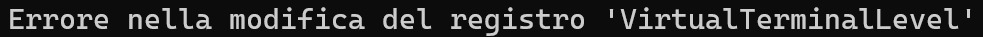
\includegraphics[width=0.8\linewidth]{Screen/erroremodificaregistro}
			\caption[Schermata principale]{}
			\label{fig:erroremodififcaregistro}
		\end{figure}
		
		
		
	\section{Schermata principale}

	
	All'avvio dell'applicazione compare la seguente schermata dove è possibile visualizzare il menu principale.
	
	\begin{figure}[H]
		\centering
		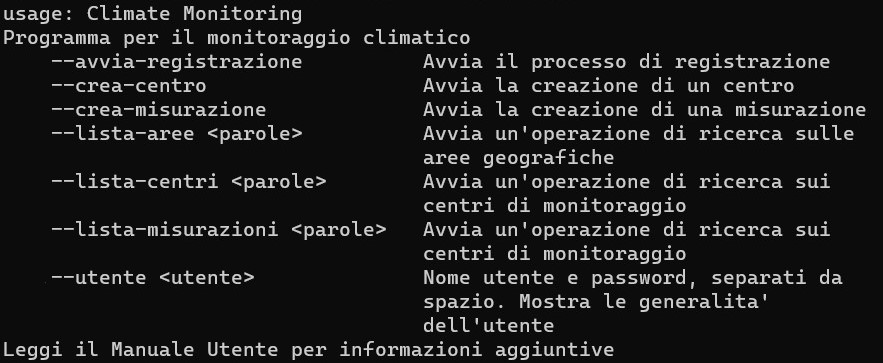
\includegraphics[width=0.9\linewidth]{Screen/schermataprincipale}
		\caption[Schermata principale]{}
		\label{fig:schermataprincipale}
	\end{figure}
	
	
		
	\section{Menù principale}
	
		\subsection{--avvia-registrazione}
		
		Per avviare questa funzione bisogna digitare il seguente comando
		\\.$\backslash$UniLab.exe --avvia-registrazione\\
		\begin{figure}[H]
			\centering
			
\includegraphics[width=0.5\linewidth]{Screen/registrazione}
			\caption[Schermata principale]{}
			\label{fig:registrazione}
		\end{figure}
				
		
		\subsection{--crea-centro}
		Per avviare questa funzione bisogna digitare il seguente comando
		\\.$\backslash$UniLab.exe --crea-centro\\
		
		\begin{figure}[H]
			\centering
			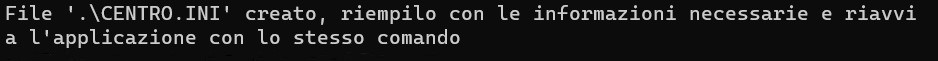
\includegraphics[width=1\linewidth]{Screen/creacentrocom}
			\caption[Schermata principale]{}
			\label{fig:creacentrocom}
		\end{figure}
		
		Una volta eseguito il comando viene creato il file "centro.ini". Bisognerà aprirlo tramite un visualizzatore di file di testo e inserire i seguenti dati:
		
		\begin{figure}[H]
			\centering
			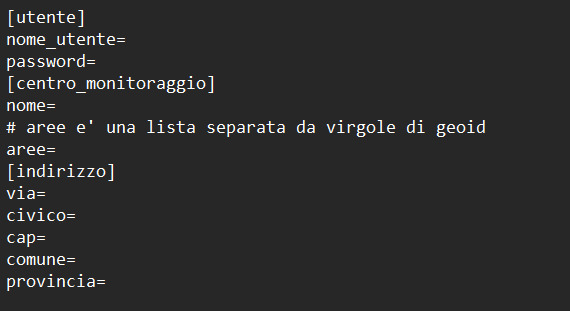
\includegraphics[width=0.8\linewidth]{Screen/creacentroini}
			\caption{}
			\label{fig:creacentroini}
		\end{figure}
		
		
		Una volta fatto ciò bisogna salvare il file e chiuderlo.
		Successivamente è necessario tornare sulla schermata del terminale e ridigitare il seguente comando:
		\\.$\backslash$UniLab.exe --crea-centro\\
		A questo punto i dati sono stati acquisiti correttamente dall'applicazione
		
		Se è già stato creato un centro e si vuole aggiungerne un altro è necessario solamente aprire il file .ini già creato e modificare i dati, salvare il file e rieseguire lo stesso comando sopracitato.
		
		
		\subsection{--crea-misurazione}
		
		Per avviare questa funzione bisogna digitare il seguente comando
		\\.$\backslash$UniLab.exe --crea-misurazione\\
		\begin{figure}[H]
			\centering
			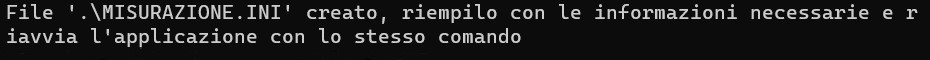
\includegraphics[width=1\linewidth]{Screen/creamisurazionecom}
			\caption[Schermata principale]{}
			\label{fig:creamisurazionecom}
		\end{figure}
		
		Una volta eseguito il comando viene creato il file "misurazione.ini". Bisognerà aprirlo tramite un visualizzatore di file di testo e inserire i seguenti dati:
		
		\begin{figure}[H]
			\centering
			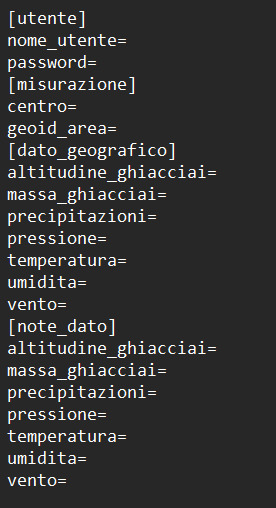
\includegraphics[width=0.4\linewidth]{Screen/creamisurazioneini}
			\caption{}
			\label{fig:creamisurazioneini}
		\end{figure}
		
		
		Una volta fatto ciò bisogna salvare il file e chiuderlo.
		Successivamente è necessario tornare sulla schermata del terminale e ridigitare il seguente comando:
		\\.$\backslash$UniLab.exe --crea-misurazione\\
		
		A questo punto i dati sono stati acquisiti correttamente dall'applicazione
		
		Se è già stata creata una misurazione e si vuole aggiungerne un'altra è necessario solamente aprire il file .ini già creato modificare i dati, salvare il file e rieseguire lo stesso comando sopracitato.
		
		
		\subsection{--lista-aree <parole>}
		Per avviare questa funzione bisogna digitare il seguente comando
		\\.$\backslash$UniLab.exe --lista-aree\\
		Questo comando permette di visualizzare tutte le aree geografiche presenti nel database.
		
		\begin{figure}[H]
			\centering
			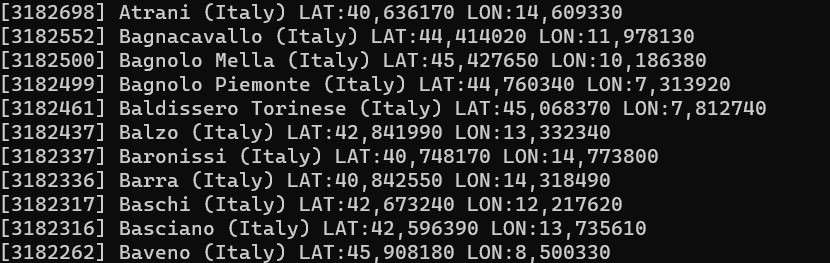
\includegraphics[width=0.9\linewidth]{Screen/listaaree}
			\caption[Schermata principale]{}
			\label{fig:listaaree}
		\end{figure}
		
		Mentre il comando
		\\.$\backslash$UniLab.exe --lista-aree <parole>\\
		Al posto di <parole>  è necessario inserire il nome dell'area geografica di interesse.
		\\Di seguito l'esempio con "mil":
		\begin{figure}[H]
			\centering
			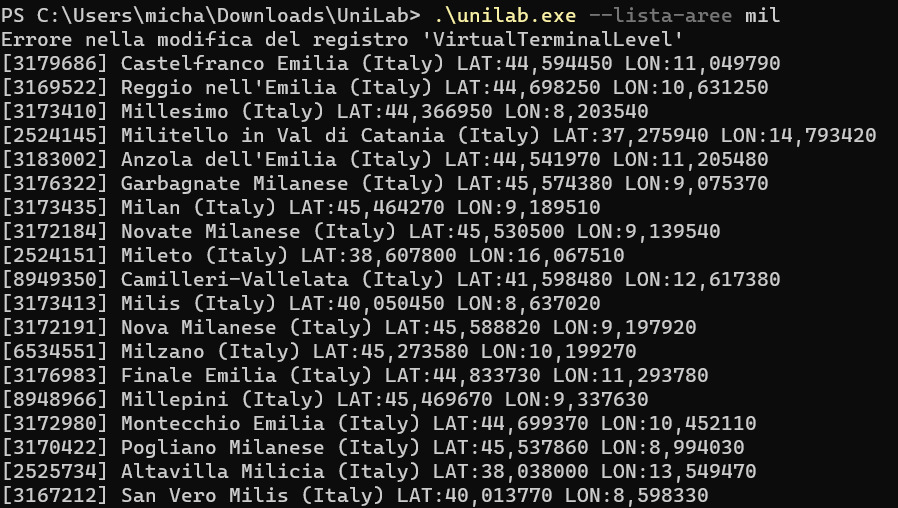
\includegraphics[width=0.9\linewidth]{Screen/listaareemil}
			\caption[Schermata principale]{}
			\label{fig:listaareemil}
		\end{figure}
		 
		
		\subsection{--lista-centri <parole>}
		
		Per avviare questa funzione bisogna digitare il seguente comando
		\\.$\backslash$UniLab.exe --lista-centri\\
		Questo comando permette di visualizzare tutti i centri di monitoraggio presenti nel database.
		
		\begin{figure}[H]
			\centering
			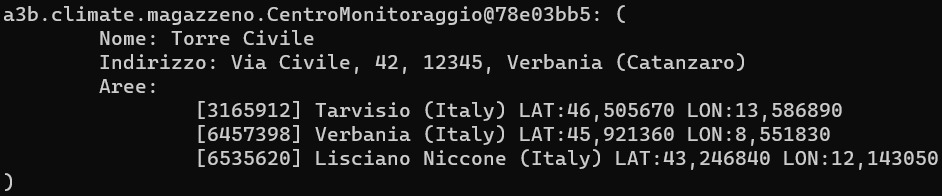
\includegraphics[width=0.9\linewidth]{Screen/listacentri}
			\caption[Schermata principale]{}
			\label{fig:listacentri}
		\end{figure}
		
		Mentre il comando
		\\.$\backslash$UniLab.exe --lista-centri <parole>\\
		Come per la precedente funzione, al posto di <parole>  è necessario inserire il nome del centro di monitoraggio di interesse.
		
		\subsection{--lista-misurazioni <parole>}
		Per avviare questa funzione bisogna digitare il seguente comando
		\\.$\backslash$UniLab.exe --lista-misurazioni\\
		Questo comando permette di visualizzare tutte le misurazioni presenti nel database.
		
		\begin{figure}[H]
			\centering
			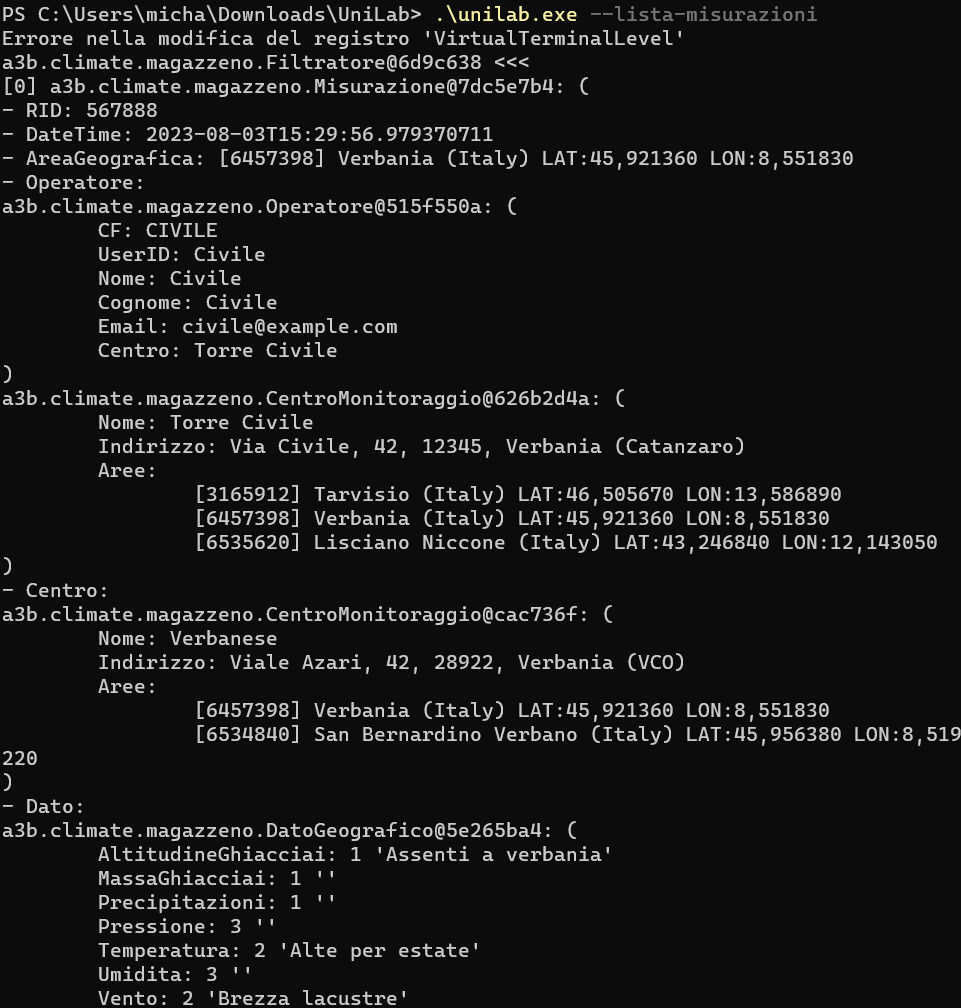
\includegraphics[width=0.9\linewidth]{Screen/listamisurazioni}
			\caption[Schermata principale]{}
			\label{fig:listamisurazioni}
		\end{figure}
		
		Mentre il comando
		\\.$\backslash$UniLab.exe --lista-misurazioni <parole>\\
		Come per la precedente funzione, al posto di <parole>  è necessario inserire la misurazione di interesse.
		
		\subsection{-u,--utente <utente>}
		Per avviare questa funzione bisogna digitare il seguente comando
		\\.$\backslash$UniLab.exe -u \\
		oppure
		\\.$\backslash$UniLab.exe --utente \\
		Questo comando permette di visualizzare il profilo dell'operatore.
		Accanto a -u bisogna inserire nome utente e password separati da spazio, come riportato nel seguente esempio:
		
		\begin{figure}[H]
			\centering
			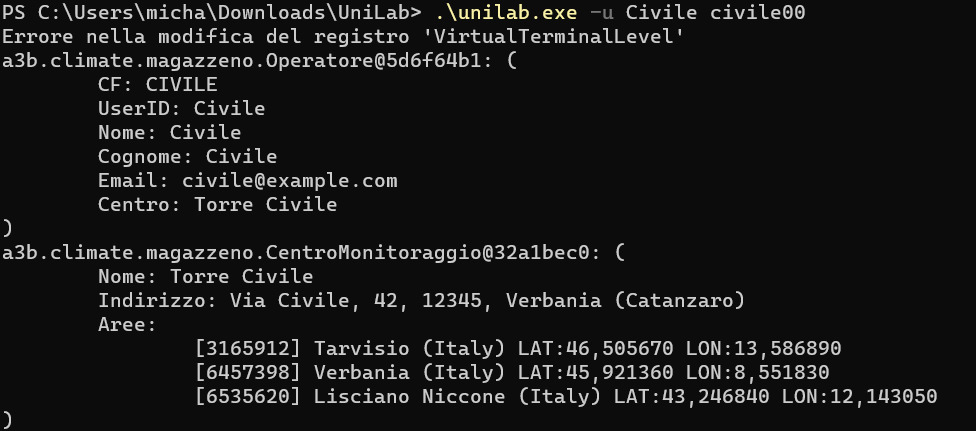
\includegraphics[width=0.9\linewidth]{Screen/utente}
			\caption[Schermata principale]{}
			\label{fig:utente}
		\end{figure}
		

	\subsection{Esci}
	Per uscire dall’applicazione è sufficiente cliccare sull’icona a croce in alto a destra

	\chapter{Limiti della soluzione sviluppata}
	Nello sviluppo dell'applicazione sono stati riscontrati alcune difficoltà nelle implementazione di alcune funzioni:
	\begin{itemize}
		\item registrazione: Il programma fornisce dei parametri di default per la registrazione in quanto non è stato possibile implementare una funzione per registrare un nuovo operatore con credenziali a scelta dall'utente.
		
		\item verifica correttezza indirizzi: Non potendo accedere direttamente al database contenente le aree geografiche, non è possibile verificare che la provincia relativa ai centri di monitoraggio sia effettivamente quella corretta.
	\end{itemize}

	
	

	\nocite{IuriTex}
	\bibliographystyle{alpha}
	\bibliography{bib/biblio}
	\printindex

\end{document}



